% Options for packages loaded elsewhere
\PassOptionsToPackage{unicode}{hyperref}
\PassOptionsToPackage{hyphens}{url}
\PassOptionsToPackage{dvipsnames,svgnames*,x11names*}{xcolor}
%
\documentclass[
  11pt,
]{article}

\usepackage{lmodern}
\usepackage{amssymb,amsmath}
\usepackage{ifxetex,ifluatex}
\ifnum 0\ifxetex 1\fi\ifluatex 1\fi=0 % if pdftex
  \usepackage[T1]{fontenc}
  \usepackage[utf8]{inputenc}
  \usepackage{textcomp} % provide euro and other symbols
\else % if luatex or xetex
  \usepackage{unicode-math}
  \defaultfontfeatures{Scale=MatchLowercase}
  \defaultfontfeatures[\rmfamily]{Ligatures=TeX,Scale=1}
  \setmainfont[]{cochineal}
  \setsansfont[]{Fira Sans}
\fi

% Use upquote if available, for straight quotes in verbatim environments
\IfFileExists{upquote.sty}{\usepackage{upquote}}{}
\IfFileExists{microtype.sty}{% use microtype if available
  \usepackage[]{microtype}
  \UseMicrotypeSet[protrusion]{basicmath} % disable protrusion for tt fonts
}{}
\makeatletter
\@ifundefined{KOMAClassName}{% if non-KOMA class
  \IfFileExists{parskip.sty}{%
    \usepackage{parskip}
  }{% else
    \setlength{\parindent}{0pt}
    \setlength{\parskip}{6pt plus 2pt minus 1pt}}
}{% if KOMA class
  \KOMAoptions{parskip=half}}
\makeatother
\usepackage{xcolor}
\IfFileExists{xurl.sty}{\usepackage{xurl}}{} % add URL line breaks if available
\IfFileExists{bookmark.sty}{\usepackage{bookmark}}{\usepackage{hyperref}}
\hypersetup{
  pdftitle={Résumé},
  pdfauthor={Nicole Rogers},
  colorlinks=true,
  linkcolor=Maroon,
  filecolor=Maroon,
  citecolor=Blue,
  urlcolor=blue,
  pdfcreator={LaTeX via pandoc}}
\urlstyle{same} % disable monospaced font for URLs
\usepackage[top=.5in, left =.5in, right=.5in, bottom=.75in]{geometry}
\setlength{\emergencystretch}{3em} % prevent overfull lines
\providecommand{\tightlist}{%
  \setlength{\itemsep}{0pt}\setlength{\parskip}{0pt}}
\setcounter{secnumdepth}{-\maxdimen} % remove section numbering

\title{Résumé}
\usepackage{authblk}
                        \author{Nicole Rogers}
            \date{12/4/2020}


%% should be top-aligned in case of uneven vertical length)
\newenvironment{columns}[1][]{}{}
%%
\newenvironment{column}[1]{\begin{minipage}[t]{#1}\ignorespaces}{%
\end{minipage}
\ifhmode\unskip\fi
\aftergroup\useignorespacesandallpars}
%%
\def\useignorespacesandallpars#1\ignorespaces\fi{%
#1\fi\ignorespacesandallpars}
%%
\makeatletter
\def\ignorespacesandallpars{%
  \@ifnextchar\par
    {\expandafter\ignorespacesandallpars\@gobble}%
    {}%
}
\makeatother

% Use fontawesome. Note: you'll need TeXLive 2015. Update.
\usepackage{fontawesome}

% Mess with sections
\usepackage{titlesec}
\usepackage{sectsty}
% \sectionfont{\rmfamily\mdseries\large\bf\underline}
\sectionfont{\normalfont\sffamily\large\bfseries\sectionrule{0pt}{0pt}{-4pt}{1pt}}
\subsectionfont{\rmfamily\mdseries\normalsize\scshape}
\titlespacing\section{0pt}{12pt plus 4pt minus 2pt}{4pt plus 2pt minus 2pt}
\titlespacing\subsection{0pt}{12pt plus 4pt minus 2pt}{4pt plus 2pt minus 2pt}

\usepackage{enumitem}
\setlist[itemize]{leftmargin=*}

\usepackage{graphicx}
\usepackage{tikz}
\usepackage{tikzpagenodes}
\usetikzlibrary{calc} 


% Make AP style (kinda) dates for the updated/today field

\usepackage{datetime}
\newdateformat{apstylekinda}{%
  \shortmonthname[\THEMONTH]. \THEDAY, \THEYEAR}

% Fancyhdr, as I tend to do with these personal documents.
\usepackage{fancyhdr,lastpage}
\pagestyle{fancy}
\renewcommand{\headrulewidth}{0.0pt}
\renewcommand{\footrulewidth}{0.0pt}
\lhead{}
\chead{}
\rhead{}
\lfoot{
\cfoot{\scriptsize  Nicole Rogers - Résumé - \emph{Updated:} \apstylekinda\today }}
\rfoot{\scriptsize \thepage/{\hypersetup{linkcolor=black}\pageref{LastPage}}}



% Always load hyperref last.
\usepackage{hyperref}
\PassOptionsToPackage{usenames,dvipsnames}{color} % color is loaded by hyperref

\hypersetup{unicode=true,
            pdftitle={Nicole Rogers  (R\'{e}sum\'{e})},
            pdfauthor={Nicole Rogers},
            colorlinks=true,
            linkcolor=Maroon,
            citecolor=Blue,
            urlcolor=blue,
            breaklinks=true, bookmarks=true}

\begin{document}
% shift=(current page.north east)
%\begin{wrapfigure}{r}{\textwidth}

\begin{tikzpicture}[remember picture,overlay, shift={(7in,-0.25in)}]
    \clip (0,0) circle (2.00cm) node {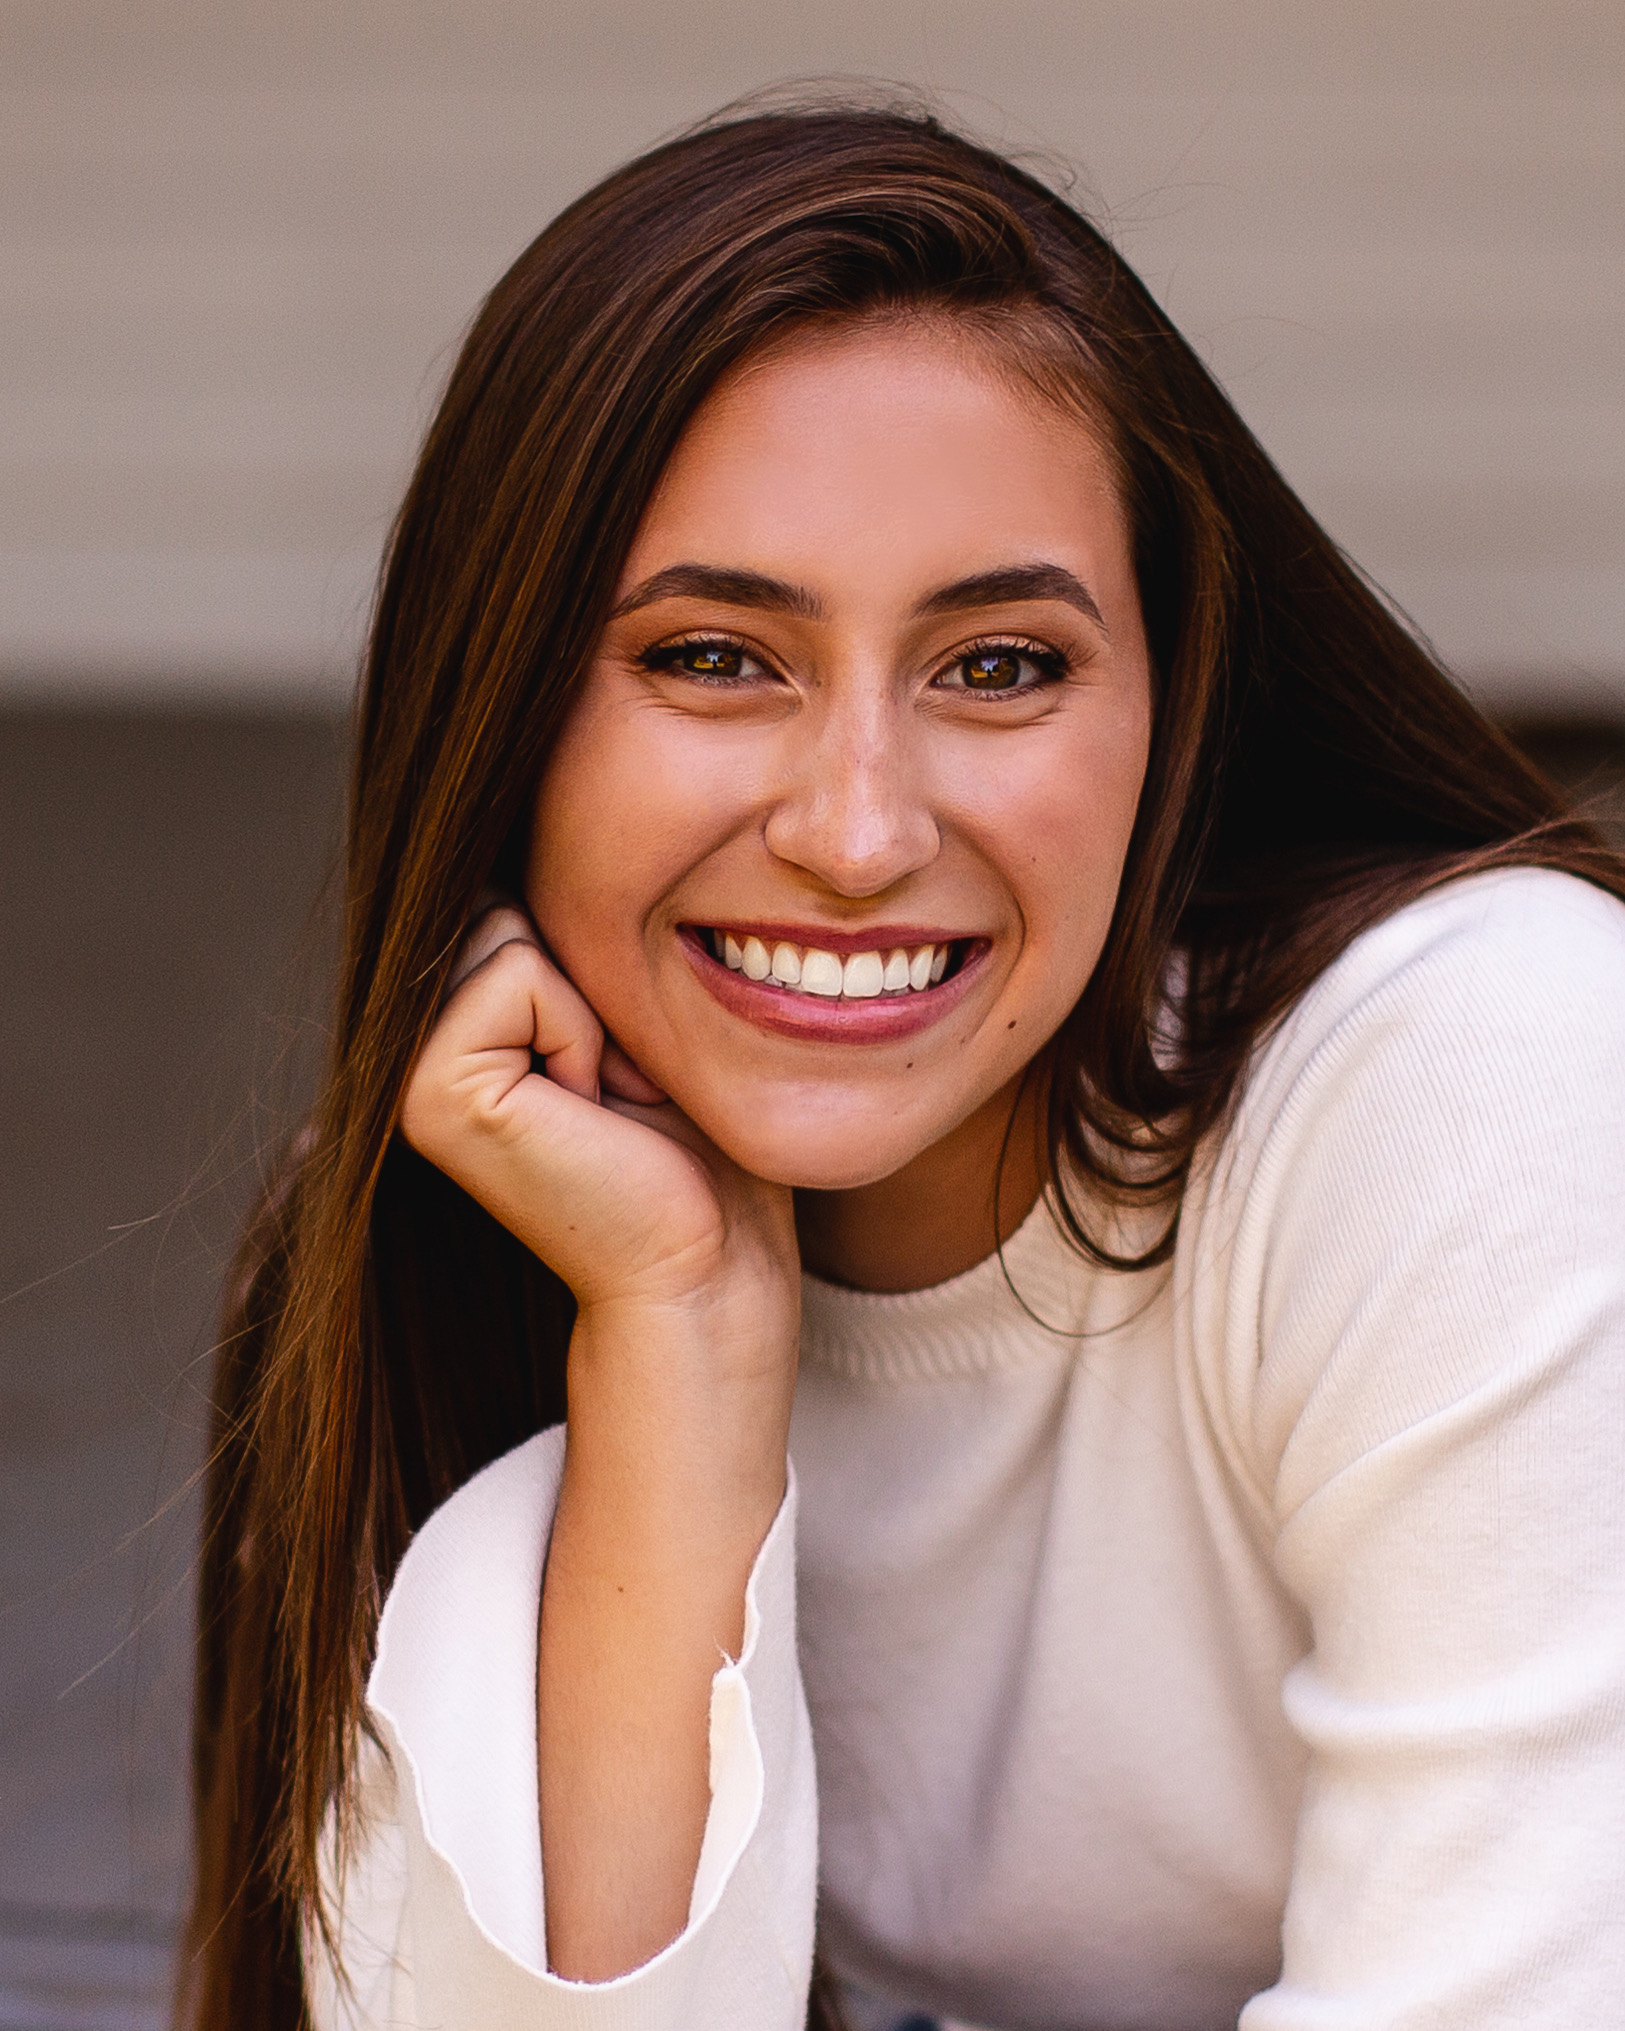
\includegraphics[width=.2\textwidth]{NicoleRogers.jpeg}};
\end{tikzpicture}

 % includephoto
%\end{wrapfigure}

\flushleft{\huge \bfseries Nicole Rogers}

\flushleft{\footnotesize

\faEnvelopeO \hspace{1 mm} \href{mailto:}{\tt \href{mailto:ntrogers@uark.edu}{\nolinkurl{ntrogers@uark.edu}}} \hspace{1 mm}
\faPhone \hspace{1 mm} 206-465-0497 \hspace{1 mm}
\faMapMarker \hspace{1 mm} Fayetteville, AR \hspace{1 mm}
}
\vspace{-1em}
\flushleft{\footnotesize
\faGlobe \hspace{1 mm} \href{http://ntrogers.netlify.app/}{\tt ntrogers.netlify.app/}  \hspace{1 mm} 
\faTwitter \hspace{1 mm} \href{http://twitter.com/}{\tt } \hspace{1 mm}
\faLinkedin \hspace{1 mm} \href{https://www.linkedin.com/in/nicole-rogers-64889a1ba}{\tt nicole-rogers-64889a1ba} \hspace{1 mm}
\faGithub \hspace{1 mm} \href{http://github.com/ntrogers}{\tt ntrogers} \hspace{1 mm}
}

\begin{column}{0.60\textwidth}

\hypertarget{professional-experience}{%
\section{Professional Experience}\label{professional-experience}}

\hypertarget{personal-tutor}{%
\subsection{Personal Tutor}\label{personal-tutor}}

\begin{itemize}
\tightlist
\item
  2019-2020 School Year
\item
  Assited learning of student in math foundations and applications
\item
  Worked directly with a profesional tutor to ensure that the most
  helpful and effective teaching styles were being used
\end{itemize}

\hypertarget{grade-8-ussf-soccer-referee}{%
\subsection{Grade 8 USSF Soccer
Referee}\label{grade-8-ussf-soccer-referee}}

\begin{itemize}
\tightlist
\item
  March 2016-August 2020
\item
  Effectively managed various players and coaches throughout the game.
\item
  Worked collaboratively with other referees to take a team approach to
  managing the game.
\item
  Mentored by various referees at the Grade 5 level and referee
  assigners.
\end{itemize}

\hypertarget{volunteering}{%
\subsection{Volunteering}\label{volunteering}}

\begin{itemize}
\tightlist
\item
  Northwest Children's Outreach: specialized in maintaining warehouse
  and creating personalized bags of clothing, books, and other
  necessities for children
\item
  Thirst Project: created and implemented a fundraisng plan to raise
  money to help build wells in developing communities in hopes to end
  the water crisis.
  \href{https://www.thirstproject.org/about/our-mission/}{Learn more
  about the Thirst Project}
\end{itemize}

\hypertarget{other-activities}{%
\subsection{Other Activities}\label{other-activities}}

\begin{itemize}
\tightlist
\item
  Model United Nations: researched and presented as a select country.
  Incited team work and collaboration to help pass resolutions.
\item
  DECA: Practiced career skills with a focus in brand marketing,
  hospitality, and entrepreneurship. Qualified for International Career
  Development Conference.
\end{itemize}

\end{column}

\begin{column}{0.02\textwidth}

~

\end{column}

\begin{column}{0.38\textwidth}

\hypertarget{education}{%
\section{Education}\label{education}}

\hypertarget{undergraduate-program}{%
\subsection{Undergraduate Program}\label{undergraduate-program}}

Attending the University of Arkansas as an Honors Fellow with a major in
Data Science

\hypertarget{high-school}{%
\subsection{High School}\label{high-school}}

Distinguished Scholar Graduate from Lakeridge High School. 4.0
unweighted GPA

\hypertarget{awards-and-positions}{%
\section{Awards and Positions}\label{awards-and-positions}}

\hypertarget{awards}{%
\subsection{Awards}\label{awards}}

\begin{itemize}
\tightlist
\item
  Merit Award for Academic Excellence (2020)
\item
  Seal of Biliteracy for Spanish (2020)
\item
  National AP Scholar (2020, 2019)
\item
  Merit Awards : Math and Social Studies (2020)
\item
  Gold Key in Scholastic Writing Competition: Poetry (2018)
\end{itemize}

\hypertarget{positions}{%
\subsection{Positions}\label{positions}}

\begin{itemize}
\tightlist
\item
  President of Lakeridge's Key Club Chapter: an international
  volunteering organization for high school students. Increased
  participation and member levels, became the largest chapter in our
  division.
\item
  Vice President of National Spanish Honors Society: managed and engaged
  with members to promote excellency in learning the language and
  increased understanding and interaction with Spanish studies
\end{itemize}

\end{column}

\end{document}

